\documentclass[paper=letter, fontsize=12pt]{article}
\usepackage{geometry}
\geometry{margin=1in}
\usepackage{graphicx}
\graphicspath{{images/}}
\usepackage{amssymb}
\usepackage{enumitem}
\usepackage{amsmath}
\usepackage{mathrsfs}

%opening
\title{Compsci 571 HW4}
\author{Yilin Gao (yg95)}

\begin{document}

\maketitle
\section{Constructing Kernels}
Let $K_1$ be kernels over $\mathbb{R}^n\times\mathbb{R}^n$, let $a \in \mathbb{R}$, $<a,b>$ denotes the dot product, $a^Tb$. .

\begin{enumerate}[label=(\alph*)]
	% 1a
	\item $K(x,z)=aK_1(x,z)$
	
	This is not a kernel. Because $K_1$ is a valid kernel, $K_1(x, z) \geq 0$. When $a < 0$, $K(x,z)=aK_1(x,z) \leq 0$. Because inner products $<\cdot, \cdot> \geq 0$, there won't be an inner product such that $K(x, z) = <\Phi(x), \Phi(z)>_{H_k}$.
	
	% 1b
	\item $K(x,z)=<x,z>^3+(<x,z>-1)^2$
	
	This is not a valid kernel. 
	
	From lecture notes we've proved $<x,z>^3$ can be expressed as inner product in a new vector space, thus a valid kernel. 
	
	For $(<x,z>-1)^2$:
	
	$(<x,z>-1)^2 = (x^T z - 1)^2 = (\sum_{i = 1}^{n} x^{(i)} z^{(i)} - 1) (\sum_{j = 1}^{n} x^{(j)} z^{(j)} - 1) = \sum_{i = 1}^{n}\sum_{j = 1}^{n} x^{(i)} x^{(j)} z^{(i)} z^{(j)} - 2 \sum_{i = 1}^{n}x^{(i)} z^{(i)} + 1 = \sum_{i = 1}^{n}\sum_{j = 1}^{n} x^{(i)} x^{(j)} z^{(i)} z^{(j)} -  \sum_{i = 1}^{n} (\sqrt{2}x^{(i)})  (\sqrt{2} z^{(i)}) + 1$
	
	This equation cannot be expressed as an inner product of some $\Phi(x)$ and $\Phi(z)$. So $(<x,z>-1)^2$ is not a valid kernel.
	
	From lecture notes we know that when $k(x, z) = k_1(x, z) + k_2(x, z)$, only if both $k_1(x, z)$ and $k_2(x, z)$ are valid kernels, will $k(x, z)$ be a valid kernel. So in this case $K(x, z)$ is not a kernel.
	
	% 1c
	\item $K(x,z)=<x,z>^2+\exp(-\|x\|^2)\exp(-\|z\|^2)$
	
	This is a valid kernel.
	
	From lecture notes we've proved $<x,z>^2$ can be expressed as inner product in a new vector space, thus a valid kernel. 
	
	From lecture notes we've proved $k(x, z) = g(x)g(z)$, $g: \mathbb{R}^n \rightarrow \mathbb{R}$ is a valid kernel, so $\exp(-\|x\|^2)\exp(-\|z\|^2)$, in the same form, is a valid kernel.
	
	So $K(x,z)=<x,z>^2+\exp(-\|x\|^2)\exp(-\|z\|^2)$, a sum of two valid kernels, is  a valid kernel.
	 
\end{enumerate}

\section{Reproducing Kernel Hilbert Spaces}

For $\mathscr{F}$ to be the RKHS for kernel $K(x,y)=xy$, it should satisfy:

\begin{enumerate}
	\item $K(x,y)$ spans $\mathscr{F}$, i.e., $\mathscr{F} = span\{ K(\cdot, x), x \in [0, 1] \} = \{f: f(\cdot) = \sum_{i = 1}^{m} \alpha_i K(\cdot, x_i), \}$
	
	\item $K(x, y)$ has the reproducing kernel property: $f(x) = <f(\cdot), K(\cdot, x)>_{\mathscr{F}_K}$
\end{enumerate}

 If $\mathscr{F}$ satisfies condition 1, for any function $f(x) = ax$ in $\mathscr{F}$, $f(x) = \sum_{i = 1}^m \alpha_i K(x, x_i)  = \sum_{i = 1}^m \alpha_i x x_i = (\sum_{i = 1}^m \alpha_i x_i ) x$, and this means the real number $a = \sum_{i = 1}^m \alpha_i x_i $ for the specific $m$ and $\alpha_i$.

 Under this condition, for any $f(\cdot) = a\cdot = (\sum_{i = 1}^m \alpha_i x_i) \cdot$, $<f(\cdot), K(\cdot, x)>_{\mathscr{F}_K} = <\sum_{i = 1}^m \alpha_i K(\cdot, x_i), K(\cdot, x)>_{\mathscr{F}_K} = \sum_{i = 1}^m \alpha_i K(x, x_i) = \sum_{i = 1}^m \alpha_i x x_i = (\sum_{i = 1}^m \alpha_i x_i) x = ax = f(x)$. So condition 2 is also satisfied.

So $\mathscr{F}$ is the RKHS for  kernel $K(x,y)=xy$. $\square$

\section{Convexity and KKT Conditions}

\begin{enumerate}[label=(\alph*)]
	% 3a
	\item
	The Lagrangian function for the primal form is:
	
	$$
	\min L(\mathbf{w}, \mathbf{\eta}, \mathbf{\eta^*}, \mathbf{a}, \mathbf{b}, \mathbf{c}, \mathbf{d}) = \frac{1}{2} \Vert \mathbf{w} \Vert^2 + C \sum_{i = 1}^{n} (\eta_i + \eta_i^*) + \sum_{i = 1}^{n} a_i [y_i - \mathbf{w}^T \mathbf{x}_i - \epsilon - \eta_i]
	$$
	
	$$
	+ \sum_{i = 1}^{n} b_i[\mathbf{w}^T \mathbf{x}_i - y_i - \epsilon - \eta_i^*] - \sum_{i = 1}^{n} c_i \eta_i - \sum_{i = 1}^{n} d_i \eta_i^*
	$$
	
	It's KKT conditions are:
	
	\begin{itemize}
		\item Primal feasibility: 
		
		$$y_i - \mathbf{w}^T \mathbf{x}_i - \epsilon - \eta_i \leq 0, i = 1, \dots, n$$
		$$\mathbf{w}^T \mathbf{x}_i  - y_i - \epsilon - \eta_i^* \leq 0, i = 1, \dots, n$$
		$$\eta_i \geq 0, i = 1, \dots, n$$
		$$\eta_i^* \geq 0, i = 1, \dots, n$$ 
		
		\item Dual feasibility:
		
		$$a_i \geq 0, i = 1, \dots, n$$
		$$b_i \geq 0, i = 1, \dots, n$$
		$$c_i \geq 0, i = 1, \dots, n$$
		$$d_i \geq 0, i = 1, \dots, n$$
		
		\item Complementary slackness:
		
		$$a_i [y_i - \mathbf{w}^T \mathbf{x}_i - \epsilon - \eta_i] = 0,  i = 1, \dots, n$$
		$$b_i [\mathbf{w}^T \mathbf{x}_i  - y_i - \epsilon - \eta_i^*] = 0,  i = 1, \dots, n$$
		$$c_i \eta_i = 0,  i = 1, \dots, n$$
		$$d_i \eta_i^* = 0,  i = 1, \dots, n$$
		
		\item Lagrangian stationary:
		
		$$\nabla_{\mathbf{w} L} = \mathbf{w} - \sum_{i = 1}^{n} (a_i - b_i) \mathbf{x}_i = 0$$
		$$(\nabla_{\mathbf{\eta} L})_{i} = C - a_i - c_i = 0, i = 1, \dots, n$$
		$$(\nabla_{\mathbf{\eta^*} L})_{i} = C - b_i - d_i = 0, i = 1, \dots, n$$

	\end{itemize} 

	With these conditions, we can transform Lagrangian function into dual form:
	
	$$
	\max L(\mathbf{a}, \mathbf{b}) = \sum_{i = 1}^{n} (a_i - b_i) y_i - \epsilon \sum_{i = 1}^{n} (a_i + b_i) - \frac{1}{2} \sum_{i, j = 1}^{n} (a_i - b_i) (a_j - b_j) \mathbf{x}_i^T \mathbf{x}_j
	$$
	
	subject to 
	$$
	0 \leq a_i, b_i \leq C, i = 1, \dots, n
	$$
	
	% 3b
	\item
	Support vectors are the points $i$ such that $\vert y_i - \mathbf{w}^T \mathbf{x}_i \vert \geq \epsilon$.
	
	% 3c
	\item
	Increasing $\epsilon$ makes the model less likely to overfit. Because the model penalizes the points that have training error larger than $\epsilon$. If $\epsilon$ increases, the allowed/unpenalized training error increases, and the model tends to overfit less.
	
	% 3d
	\item
	Increasing $C$ makes the model more likely to overfit. $C$ is the penalty for each point that has training error larger than $\epsilon$. If the penalty increases, the model will try to make points have smaller training error, and thus overfits.
	
	% 3e
	\item    
	Assume we've computed the optimal dual variables as $\mathbf{a}^*$ and $\mathbf{b}^*$.
	
	From one of the KKT conditions, we can get the optimal primal variable is $\mathbf{w}^* = \sum_{i = 1}^{n} (a_i^* - b_i^*) \mathbf{x}_i$ .
	
	So for a new point $\mathbf{x}^{new}$, its evaluation is $f(\mathbf{x}^{new}) = \sum_{j = 1}^{p} w_j^* x_j^{new} = \sum_{j = 1}^{p} \sum_{i = 1}^{n} (a_i^* - b_i^*) x_{ij} x_j^{new} = \sum_{i = 1}^{n} (a_i^* - b_i^*) \mathbf{x}_i \cdot \mathbf{x}^{new }$.
\end{enumerate}

\section{SVM Implementation}
\begin{enumerate}[label=(\alph*)]
	%4a
	\item See \texttt{svm\_classifier.py}.
	
	%4b
	\item \textbf{Note: for questions (b) and (c), I use \texttt{sklearn.mode\_selection.train\_test\_split} to split the training and testing set with 2018 as the random seed. And if I use \texttt{numpy} with 2018 as the random seed to generate indices for training and testing data and then split, the split is different.} Code for these 2 questions are in \texttt{q4.ipynb}.
	
	The accuracy of the classifier on testing data is 0.8636363636363636. The ROC curve is like following:
	
	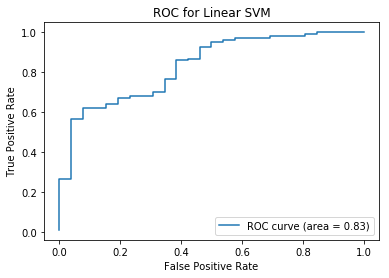
\includegraphics[scale=0.6]{q4b.png}
	
	The AUC on testing data is 0.8316400580551523.
	
	%4c
	\item For $\sigma^2 = 25$, the accuracy of the classifier on testing data is 0.8484848484848485. The ROC curve is like:
	
	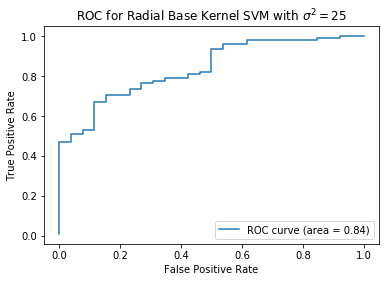
\includegraphics[scale=0.6]{q4c1.png}
	
	The AUC on testing data is 0.8388969521044993.
	
	For $\sigma^2 = 5$, the accuracy for the classifier on testing data is 0.7954545454545454. The ROC curve is like:
	
	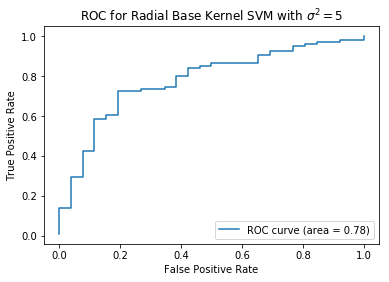
\includegraphics[scale=0.6]{q4c2.png}

	The AUC on testing data is 0.7790275761973875.
	
	The comparison between 2 $\sigma^2$ values suggests that for Gaussian kernel if we set $\sigma^2$ too small we may overfit.
\end{enumerate}

\end{document}
